\documentclass[10pt, a4paper, italian]{article}
\usepackage[T1]{fontenc}
\usepackage[utf8]{inputenc}
\usepackage{amsmath, amssymb, amsthm, thmtools, amsfonts, mathtools}
\usepackage{nicefrac}
\usepackage{calc}
\usepackage[pdftex, hyperindex, plainpages=false]{hyperref}
\usepackage[nameinlink]{cleveref} %load before classicthesis (clash)
%\usepackage[nochapters,pdfspacing]{classicthesis}
\usepackage{siunitx}
\usepackage[siunitx]{circuitikz}

\usepackage[a4paper]{geometry}
\usepackage{float}
\usepackage{mdframed}
\usepackage{titling}
\usepackage{booktabs}
\usepackage{graphicx}
\usepackage{caption, subcaption}
\usepackage{xcolor}
\usepackage[italian]{babel}
\usepackage{pgfplots}
\usepackage{listings}
%\usepackage{lmodern}
\usepackage{url}
\usepackage{enumitem}
\usepackage{tikz} %loads after classicthesis (xcolor incompat)

% lets graphicx know path where figures to be included are found
\graphicspath{{../figs/}}
\makeatletter
\def\input@path{{../figs/}}
%or: \def\input@path{{/path/to/folder/}{/path/to/other/folder/}}
\makeatother

% tikz pgf plots setup
\usepgfplotslibrary{external}
\pgfplotsset{compat=1.15}
%\tikzexternalize

% spaces and significant digits/figures for measurements
\sisetup{free-standing-units, space-before-unit, number-unit-product = \;,
scientific-notation = false, round-mode = figures, round-precision = 1,}

% turns all (hyperlinked) references black [default is blue]
\hypersetup{
	linktoc=all,
	colorlinks=true,
	linkcolor=black
}

% code listings config
%\lstset{
%language=Python,
%basicstyle=\ttfamily,
%columns=fullflexible,
%keepspaces=true,
%}

% mdframed (for boxed text) configuration
\mdfsetup{linewidth=0.6pt}

% Default fixed font does not support bold face
\DeclareFixedFont{\ttb}{T1}{txtt}{bx}{n}{12} % for bold
\DeclareFixedFont{\ttm}{T1}{txtt}{m}{n}{12}  % for normal

% Custom colors
\usepackage{color}
\definecolor{deepblue}{rgb}{0,0,0.5}
\definecolor{deepred}{rgb}{0.6,0,0}
\definecolor{deepgreen}{rgb}{0,0.5,0}

% Commands 
\newcommand{\executeiffilenewer}[3]{%
	\ifnum\pdfstrcmp{\pdffilemoddate{#1}}%
		{\pdffilemoddate{#2}}>0%
	{\immediate\write18{#3}}\fi%
}
% input .svg --> .pdf_tex graphs
%\newcommand{\includesvg}[1]{%
%	\executeiffilenewer{#1.svg}{#1.pdf}%
%	{inkscape -z -D --file=#1.svg %
%	--export-pdf=#1.pdf --export-latex}%
%	\input{#1.pdf_tex}%
%}
% Thanks UniPi's Department of Physics E. Fermi
\newcommand{\thanksdf}{(\thanks{Dipartimento di Fisica E.~Fermi,%
Universit\`a di Pisa - Pisa, Italy.}\;)}

% hyperlink to email address
\newcommand{\mail}[1]{\href{mailto:#1}{\textsf{#1}}}

% \vec for bold vectors, instead of overarrows (now "\arrvec")
\let\arrvec=\vec
\renewcommand{\vec}[1]{\boldsymbol #1}
% replaces straight phi with slanted phi
\renewcommand{\phi}{\varphi}
% replaces straight eps with curved epsilon
\newcommand{\eps}{\varepsilon}
% abbreviation for (sub_/super^)scripts of \lim, \sum,... in inline math
\newcommand{\ds}{\displaystyle}

% blackboard/number set letters
\newcommand{\CC}{\mathbb C}
\newcommand{\HH}{\mathbb H}
\newcommand{\KK}{\mathbb K}
\newcommand{\NN}{\mathbb N}
\newcommand{\PP}{\mathbb P}
\newcommand{\QQ}{\mathbb Q}
\newcommand{\RR}{\mathbb R}
\newcommand{\ZZ}{\mathbb Z}

\newcommand{\Abs}[1]{{\left\Vert #1\right\Vert}}
\newcommand{\enclose}[1]{{\left( #1 \right)}}
\newcommand{\Enclose}[1]{{\left[ #1 \right]}}
\newcommand{\floor}[1]{\left\lfloor #1 \right\rfloor}
\newcommand{\ceil}[1]{\left\lceil #1 \right\rceil}
\newcommand{\To}{\rightrightarrows}

% Math operators
\DeclareMathOperator{\divergence}{div}
\renewcommand{\div}{\divergence}
\DeclareMathOperator{\Imaginarypart}{Im}
\renewcommand{\Im}{\Imaginarypart}
\DeclareMathOperator{\Realpart}{Re}
\renewcommand{\Re}{\Realpart}
%\DeclareMathOperator{\arg}{arg}
\DeclareMathOperator{\tg}{tg}
\DeclareMathOperator{\arctg}{arctg}
\DeclareMathOperator{\settsinh}{settsinh}
\DeclareMathOperator{\settcosh}{settcosh}
\DeclareMathOperator{\tr}{tr}
\DeclareMathOperator{\im}{im}
\DeclareMathOperator{\sgn}{sgn}
\DeclareMathOperator{\diag}{diag}

\DeclarePairedDelimiter{\norm}{\lVert}{\rVert}
\DeclarePairedDelimiter{\scalar}{\langle}{\rangle}

% Logarithm with arbitrary base.
% -> log_10
\newcommand{\llog}[1][10]{\log_{#1}}

% Absolute value.
% -> |x|
\newcommand{\abs}[1]{\left| #1 \right|}

% Powers.
% -> x^a
\newcommand{\power}[2][2]{\left( #2 \right)^{#1}}

% Square.
% -> x^2
\newcommand{\sq}[1]{\power[2]{#1}}

% Expansion of the binomial coefficient.
% -> n1!/(n2!(n1 - n2)!)
\newcommand{\binomexpr}[2]{\frac{#1!}{#2!(#1 - #2)!}}

% Expression evaluation at a given point with square brackets.
% -> [x]_{a}
\newcommand{\at}[2]{\left[ #1\right]_{\makebox[-1pt][l]{${\scriptstyle#2}$}}}

% Expression evaluation in an interval.
% -> [x] _{a}^{b}
\newcommand{\eval}[3]{\left.#1%
  \right|_{\makebox[-1pt][l]{${\scriptstyle#2}$}}^{\makebox[-1pt][l]{${\scriptstyle#3}$}}}

% Upright d in math mode (for differentials).
% -> d
\newcommand{\ud}{\mathrm{d}}

% Differential.
% -> dx
\newcommand{\diff}[1][x]{\,\ud{#1}}

% Base command for defining derivatives.
% -> df/dx or d^kf/dx^k
\newcommand{\basederivative}[4][]{%
  \displaystyle%
  \ifx\\#1\\\frac{#4#2}{#4#3}%
  \else%
  \frac{#4^#1#2}{#4#3^#1}%
  \fi%
}

% Total derivative.
% -> df/dx(x) or d^kf/dx^k(x)
\newcommand{\td}[4][]{%
  \basederivative[#1]{#2}{#3}{\ud}%
  \ifx\\#4\\%
  \else%
  \mkern-4mu\left(#4\right)%
  \fi%
}

% Partial derivative.
% -> df/dx(x) or d^kf/dx^k(x)
\newcommand{\pd}[4][]{%
  \basederivative[#1]{#2}{#3}{\partial}%
  \ifx\\#4\\%
  \else%
  \mkern-4mu\left(#4\right)%
  \fi%
}

\newcommand{\intinf}{\int_{-\infty}^{\infty}\!\!\!}

\newcommand{\cinterval}[2]{\left[\, #1,~#2 \,\right]}

\newcommand{\linterval}[2]{\left[\, #1,~#2 \,\right)}

\newcommand{\rinterval}[2]{\left(\, #1,~#2 \,\right]}

\newcommand{\ointerval}[2]{\left(\, #1,~#2 \,\right)}

\newcommand{\prob}[1]{\displaystyle P\left(#1\right)}

\newcommand{\pvalue}{\emph{$p$-value}}

\newcommand{\cond}{\,|\,}

\newcommand{\expect}[1]{\displaystyle E\left[#1\right]}

\newcommand{\mom}[2][]{\displaystyle {\cal M}_{#2}\ifx\\#1\\\else(#1)\fi}

\newcommand{\momalg}[1]{\displaystyle \lambda_{#1}}

\newcommand{\momcen}[1]{\displaystyle \mu_{#1}}

\newcommand{\skewness}{\displaystyle \gamma_1}

\newcommand{\kurtosis}{\displaystyle \gamma_2}

\newcommand{\charf}[1][x]{\phi_{#1}}

\newcommand{\momgenf}[1][x]{M_{#1}}

\newcommand{\fwhm}{{\scriptstyle \textsc{FWHM}}}

\newcommand{\hwhm}{{\scriptstyle \textsc{HWHM}}}

\newcommand{\median}{\mu_{\nicefrac{1}{2}}}

\newcommand{\var}[1]{\ensuremath{\text{Var}\left(#1\right)}}

\newcommand{\cov}[2]{\ensuremath{\text{Cov}\left(#1, #2\right)}}

\newcommand{\corr}[2]{\ensuremath{\text{Corr}\left(#1, #2\right)}}

\newcommand{\like}{\mathcal L}

\newcommand{\likelihood}[2][]{\like\ifx\\#2\\\else(#2\ifx\\#1\\\else;#1\fi)\fi}

\newcommand{\chisq}{\ensuremath{\chi^2}}

\newcommand{\chisquare}[2][]{\chisq\ifx\\#2\\\else(#2\ifx\\#1\\\else;#1\fi)\fi}

\newcommand{\loglikelihood}[2][]{\log\likelihood[#1]{#2}}

\newcommand{\pdf}[3][]{#2(#3\ifx\\#1\\\else;#1\fi)}

\newcommand{\binomialpdf}[2][]{\pdf[#1]{\mathcal B}{#2}}

\newcommand{\multinomialpdf}[2][]{\pdf[#1]{\mathcal M}{#2}}

\newcommand{\poissonpdf}[2][]{\pdf[#1]{\mathcal P}{#2}}

\newcommand{\uniformpdf}[2][]{\pdf[#1]{u}{#2}}

\newcommand{\exponentialpdf}[2][]{\pdf[#1]{\varepsilon}{#2}}

\newcommand{\gausspdf}[2][]{\pdf[#1]{N}{#2}}

\newcommand{\chisquarepdf}[2][]{\pdf[#1]{\wp}{#2}}

\newcommand{\cauchypdf}[2][]{\pdf[#1]{c}{#2}}

\newcommand{\erf}[1]{\ensuremath{\text{erf}\left(#1\right)}}

\newcommand{\dccases}[4][]{#2 \ifx\\#2\\\else=\fi %
  \begin{cases}
    \displaystyle #3 & \text{per variabili discrete}\\
    \displaystyle #4 & \text{per variabili continue}#1
  \end{cases}
}
% sub/super-scriptable for all symbol as math operator 
\newcommand\Scaleforall[1]{\vcenter{\hbox{\scalefont{#1}$\forall$}}}

\DeclareMathOperator*\forevery{%
  \vphantom\sum
  \mathchoice{\Scaleforall{2}}{\Scaleforall{1.4}}{\Scaleforall{1}}{\Scaleforall{0.75}}}
\geometry{left=2cm, right=2cm, top=2cm, bottom=2cm}

% indexes subsections with letters, sections with numbers (1.a, 1.b, ...)
\renewcommand{\thesubsection}{\thesection.\alph{subsection}}

% lets graphicx know path where figures to be included are found
\graphicspath{{../figs/}}

\author{Gruppo 1.AC \\ Matteo Rossi, Bernardo Tomelleri}
\title{Es11: Esperimenti di Interferometria per misure di lunghezze d'onda}
\begin{document}
\date{\today}
\maketitle

%=======================
\section{Scopo dell'esperienza}
Lo scopo dell'esperienza è misurare la lunghezza d'onda di un laser
a semiconduttore studiando il pattern di diffrazione generato da un suo
fascio incidente sulla scala millimetrata di un calibro.

\section{Metodo di misura}
Un reticolo di diffrazione è un apparato capace di disperdere un fascio
luminoso incidente in funzione della sua lunghezza d'onda. Il fenomeno alla
base di tale separazione è l'interferenza luminosa, per la quale è possibile
determinare la seguente relazione tra lunghezza d'onda della riga spettrale
diffratta e la sua posizione angolare
\begin{equation}
d(\sin(\theta _i) - \sin(\theta _m)) = m \lambda
\label{eq: diff}
\end{equation}
in cui $m (\in \ZZ$) è l'ordine di interferenza per cui si individuano le
posizioni dei massimi principali, $\lambda$ è la lunghezza d'onda del fascio
incidente (come di quello riflesso), $\theta _m$ è l'angolo che
individua la posizioni di diffrazione relativa all'$m$-esimo ordine, $d$ è il
passo del reticolo.
L'angolo di incidenza sul reticolo viene denominato $\theta _i$.

Dalla misura degli angoli di diffrazione, noto il loro ordine e noto il passo
reticolare, possiamo individuare una relazione lineare che ci permetta di
ricavare la lunghezza d'onda come evidenziata in \cref{eq: diff}:
\begin{equation}
y = -x \frac{\lambda}{d} + q
\label{eq: fit}
\end{equation}
dove $y,x$ e $q$ sono rispettivamente $\sin(\theta _m)$, $m$ e
$\sin(\theta _i)$.

\begin{figure}
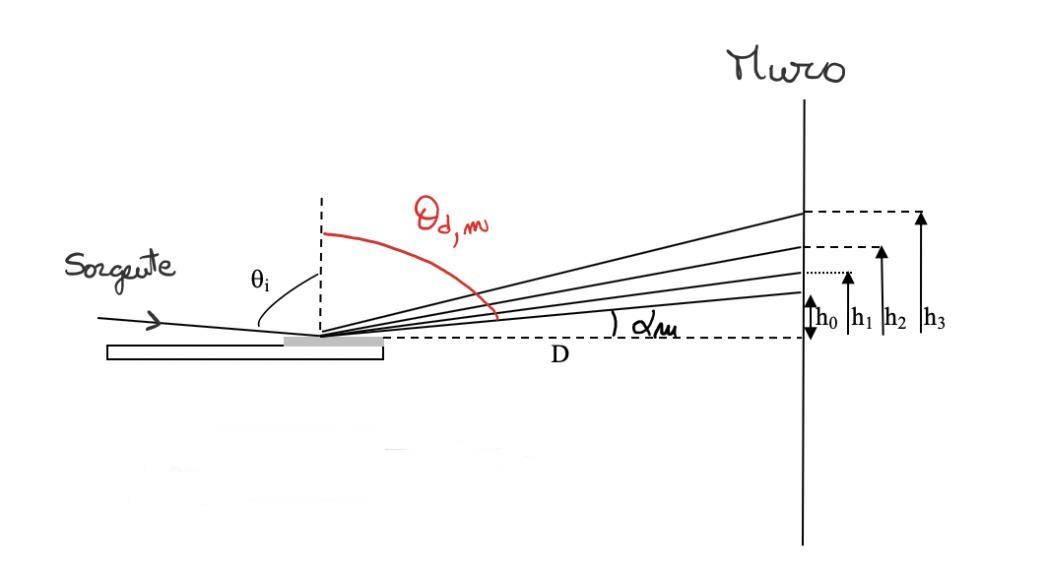
\includegraphics[width=\textwidth]{0}
\caption{Schema di riferimento dell'apparato sperimentale utilizzato
\label{fig: schema}}
\end{figure}

I valori degli angoli si intendono in riferimento al sistema che ha come
origine il punto in cui è posto il calibro, di modo da poter ricavare
direttamente come misure di altezza i massimi di diffrazione.

Infatti si vede facilmente come
\begin{equation}
\sin(\theta _m) = \frac{D}{\sqrt{D^2 + h_m^2}} = 
\left(1 + \left(\frac{h_m}{D}\right)^2\right)^{-\frac{1}{2}}
\label{eq: gon}
\end{equation}
dove $h_m$ sono le altezze relative dei massimi di diffrazione misurate
rispetto al punto di riferimento.

\subsection{Nota sul metodo di fit}
Per determinare i parametri ottimali e le rispettive covarianze si \`e
implementato in \verb+Python+ un algoritmo di fit basato sui minimi quadrati
mediante la funzione \emph{curve\_fit} della libreria \texttt{SciPy}.

\subsection{Descrizione delle misure}
Si utilizza un diodo laser con lunghezza d'onda pari a $636 \pm 1 \; \si{n\m}$
(reperibile da datasheet) che incide sul reticolo di diffrazione in
riflessione costituito dalla scala graduata di un calibro ventesimale.
Da questo sappiamo che il valore del passo reticolare è pari a
$d = 1 \; \si{m\m}$.
%TODO INCERTEZZA SUL PASSO DA COSTRUTTORE DEL CALIBRO

Noto il valore del passo reticolare, viene eseguita una stima dell'angolo di
diffrazione usando \cref{eq: fit} applicata a partire dall'ordine $m = 0$.
Per fare questo è stato prima necessario determinare la distanza tra l'origine
dei fasci e lo schermo su cui essi erano proiettati:
\[
D = 2.90 \pm 0.03 \; \si{\m}
\]
dove l'incertezza risente della larghezza dello spot del fascio proiettato,
che per l'ordine $m = 0$ corrisponde a una regione luminosa di diametro
$6.0 \pm 0.1 \; \si{c\m}$ sull'asta del calibro.
Dal momento che il fascio risulta (entro la sensibilità sperimentale)
ortogonale allo schermo e al reticolo, si trascurano possibili effetti di
distorsione e si sceglie di individuare il punto di massima intensità luminosa
al suo centro, associando alla sua posizione un'incertezza corrispondente
alla semilarghezza dell'intera regione illuminata (come si farà per le.

Successivamente si è spostato il calibro in modo che solo una porzione del fascio incidesse sulla sua scala.

Abbiamo quindi definito un valore di azzeramento per tutte le seguenti misure di
angoli, scegliendo il valore medio tra la proiezione del fascio diretto e
quello riflesso all'ordine zero. Da cui troviamo come valore stimato per
l'altezza di riferimento:
\[
h_0 = 5.3 \pm 0.1 \; \si{c\m}
\]

Abbiamo registrato le altezze di 25 massimi di diffrazione, di cui si
riportano in \cref{tab: hm} i valori dei seni degli angoli misurati $\sin{\theta_m}$
relativi al punto di azzeramento. L'incertezza associata alle misure deriva dallo
spessore non trascurabile dei singoli spot luminosi, in maniera simile a quanto
visto in precedenza per determinare la posizione dell'ordine 0.
\begin{table}[htbp]
\centering
\begin{tabular}{ccccc}
\toprule
ordine di diffrazione $m$ & $h_m \; [\si{c\m}]$ &
$\sigma (h_m) \; [\si{m\m}]$ & $\sin(\theta _m)$ & $\sigma(\sin{\theta _m})$ \\
\midrule
\midrule
0  & 5.3 & 1.0 & 1.00000 & $1 \times 10^{-6}$ \\
1  & 11.5 & 1.0 & 0.99921 & $2 \times 10^{-5}$ \\
2  & 15.5 & 1.0 & 0.99857 & $3 \times 10^{-5}$ \\
3  & 18.6 & 1.0 & 0.99795 & $5 \times 10^{-5}$ \\
4  & 21.3 & 1.0 & 0.99731 & $6 \times 10^{-5}$ \\
5  & 23.7 & 1.0 & 0.99667 & $7 \times 10^{-5}$ \\
6  & 26 & 2 & 0.9960 & $1 \times 10^{-4}$ \\
7  & 28 & 2 & 0.9954 & $1 \times 10^{-4}$ \\
8  & 30 & 2 & 0.9947 & $1 \times 10^{-4}$ \\
9  & 32 & 2 & 0.9941 & $1 \times 10^{-4}$ \\
10 & 33 & 2 & 0.9935 & $2 \times 10^{-4}$ \\
11 & 35 & 2 & 0.9929 & $2 \times 10^{-4}$ \\
12 & 36 & 2 & 0.9922 & $2 \times 10^{-4}$ \\
13 & 38 & 2 & 0.9916 & $2 \times 10^{-4}$ \\
14 & 39 & 2 & 0.9909 & $2 \times 10^{-4}$ \\
15 & 41 & 3 & 0.9903 & $2 \times 10^{-4}$ \\
16 & 42 & 3 & 0.9897 & $3 \times 10^{-4}$ \\
17 & 43 & 3 & 0.9890 & $3 \times 10^{-4}$ \\
18 & 44 & 3 & 0.9884 & $3 \times 10^{-4}$ \\
19 & 46 & 2 & 0.9877 & $3 \times 10^{-4}$ \\
20 & 47 & 2 & 0.9871 & $3 \times 10^{-4}$ \\
21 & 48 & 2 & 0.9865 & $3 \times 10^{-4}$ \\
22 & 49 & 2 & 0.9858 & $3 \times 10^{-4}$ \\
23 & 50 & 2 & 0.9852 & $3 \times 10^{-4}$ \\
24 & 51 & 1 & 0.9846 & $3 \times 10^{-4}$ \\
25 & 52 & 1 & 0.9841 & $3 \times 10^{-4}$ \\
\bottomrule
\end{tabular}
\caption{Misure delle altezze delle proiezioni dei fasci riflessi e
corrispondenti seni degli angoli associati al variare degli ordini di
diffrazione. \label{tab: hm}}
\end{table}

A questo punto si effettua un fit lineare sulla base dell'\cref{eq: fit},
da cui è possibile stimare il coefficiente angolare $\frac{\lambda}{d}$ e
dunque $\lambda$ della radiazione emessa.

Dalla procedura di fit viene escluso il valore $h_0$ al fine di verificare che
l'intercetta risultasse compatibile con questo.
Data l'origine sistematica degli errori sulle misure di distanza $D$ e delle
posizioni dei centri dei massimi di diffrazione abbiamo impostato il flag
\verb+absolute_sigma=True+ in modo che la funzione curve\_fit non riscalasse
le incertezze fornite in ingresso.

\begin{figure}
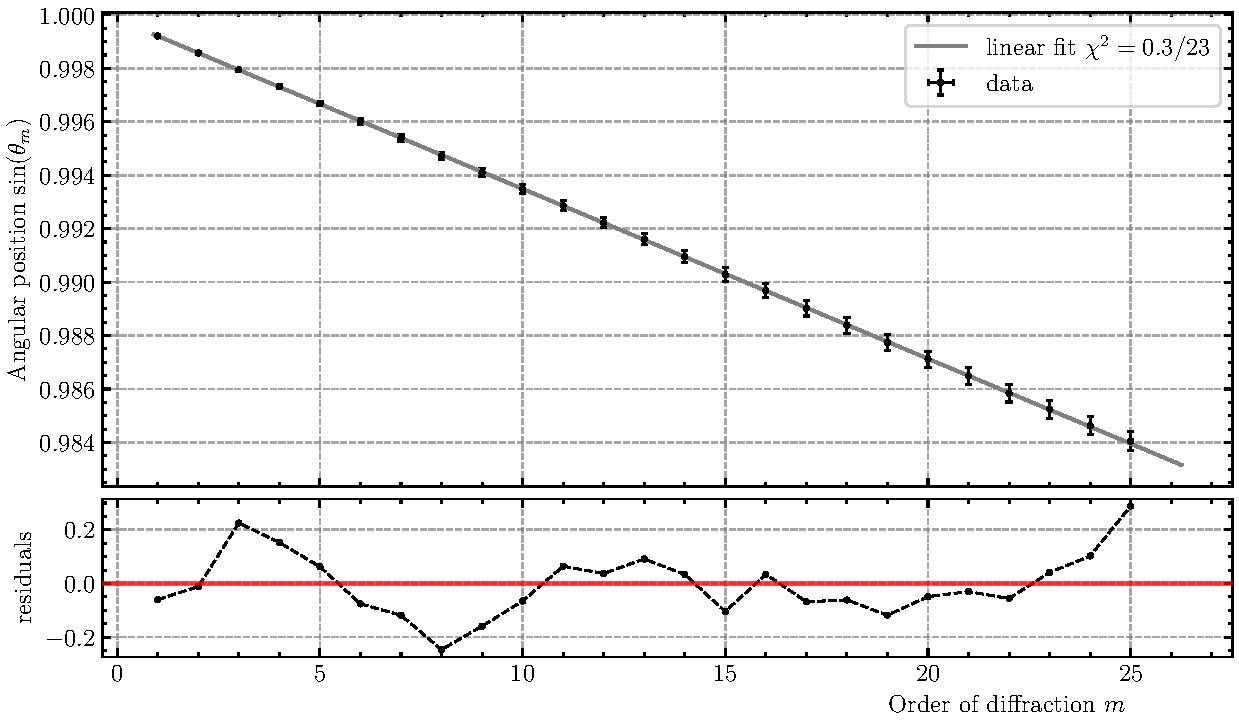
\includegraphics[width=\textwidth]{thetafit}
\caption{Grafico della retta di best-fit e residui normalizzati per
l'andamento delle posizioni angolari $\sin{\theta_m}$ in funzione dell'ordine
di diffrazione $m$. Il grafico dei residui non evidenzia nessun andamento
che devii in maniera sistematica dal modello utilizzato (\cref{eq: fit}).
\label{fig: linfit}}
\end{figure}

\begin{table}
\centering
\begin{tabular}{ccccc}
\toprule
$\lambda/d$ [arb. un.] & $\sin{\theta_i}$ [arb. un.] &
$\chi^2/\text{ndof}$ & norm. cov. \\
\midrule
$(636 \pm 1) \; \times 10^{-6}$ & $(999.8 \pm 0.2) \; \times 10^{-3}$ &
$0.3/23$ & $-0.99$ \\
\bottomrule
\end{tabular}
\caption{Risultati del fit lineare per la misura del rapporto $\lambda/d$
\label{tab: linfit}}
\end{table}

Dal fit ricaviamo quindi (moltiplicando per il passo reticolare noto) che
$\lambda = 635.7 \pm 0.5 \; \si{n\m}$, che il valore ottimale di $\theta_i$
risulta compatibile con $\pi/2$ entro l'incertezza e che la nostra misura di
$\lambda$ risulta in ottimo accordo con quanto tabulato nel datasheet del
laser.

%=======================
\section{Interferometro di Michelson: lunghezza d'onda della lampada Hg}
\subsection{Stima del fattore di demoltiplica}
Per calibrare l'apparato e stimare il fattore di demoltiplica tra lo
spostamento del nonio della vite micrometrica e lo spostamento dello
specchio mobile M1 è stato utilizzato un laser He-Ne di lunghezza d'onda nota
($632.8 \; \si{n\m}$).
Per prima cosa si è calibrata la posizione dello specchio M2 in modo che sul
centro dello schermo apparisse un pattern circolare di interferenza dovuto
allo sfasamento tra i 2 fasci di luce prodotto dai diversi cammini ottici
lungo i bracci dell'interferometro.
Una volta fissata la posizione di M2 abbiamo iniziato a variare la distanza
di M1 contando il numero di fronti d'onda passanti da un punto qualunque
sullo schermo (per comodità il centro) in funzione dello spostamento
effettuato dalla vite di M1. 

Il fattore di demoltiplica $\kappa$ si può stimare a partire dall'equazione
fondamentale tra il numero di frange $m$ che si vedono passare per il centro
$m$ e lo spostamento $\Delta L$ del braccio dello specchio M1
\begin{equation}\label{eq: fond}
2 \Delta L = m \lambda
\end{equation}
tramite l'equazione
\begin{equation}\label{eq: dem}
\kappa = \frac{m \lambda}{2 \Delta L}
\end{equation}

Ripetendo la misura al variare degli spostamenti $Delta L$ 2 volte abbiamo
ottenuto 
\[
\def\arraystretch{1.5}
\begin{array}{rcl}
\kappa_1 & = & 198 \pm 9 \times 10^{-3} \\
\kappa_2 & = & 0.21 \pm 0.01 \\
\end{array}
\]
facendo poi la media pesata delle misure si è ricavata la nostra stima
ottimale del fattore di conversione
$\kappa = 206 \pm 8 \; \times 10^{-3}$.

\subsubsection{Misura della lunghezza d'onda della lampada Hg}
Manipolando l'\cref{eq: dem} si arriva alla formula usata per la misura della
lunghezza d'onda di una sorgente in funzione del numero dei fronti
d'onda $m$, del fattore di demoltiplica $\kappa$ e dello spostamento effettuato
dalla vite micrometrica $\Delta L$.
\[
\lambda = \frac{2 \Delta L \kappa}{m}
\]
Abbiamo quindi sostituito la sorgente di radiazione luminosa con una lampada
al mercurio di lunghezza d'onda attesa $\lambda\ped{exp} = 546 \; \si{n\m}$;
dopodiché, seguendo la stessa procedura di prima abbiamo contato i fronti
d'onda in funzione dello spostamento della vite micrometrica, da cui troviamo
\[
\def\arraystretch{1.5}
\begin{array}{rcl}
\lambda_1 & = & 5.5 \pm 0.4 \times 10^{-7} \; \si{m} \\
\lambda_2 & = & 5.4 \pm 0.4 \times 10^{-7} \; \si{m} \\
\end{array}
\]

Di nuovo da una media pesata delle due misure si è ottenuta la nostra miglior
stima della lunghezza d'onda $\lambda\ped{Hg} = 545 \pm 28 \; \si{n\m}$ che
risulta compatibile con le aspettative.

%=======================
\section*{Conclusioni e commenti finali}
Siamo riusciti a stimare la lunghezza d'onda di un laser a diodo utilizzando
come reticolo di diffrazione in riflessione un calibro ventesimale.
Dunque, utilizzando un interferometro di Michelson si è ottenuta una misura
ragionevole della lunghezza d'onda di una lampada al mercurio.
Le misure di queste grandezze sono affette da diverse sorgenti di errore non
trascurabili, principalmente dovute alla difficoltà nell'individuare posizioni
esatte per le immagini dei fenomeni luminosi studiati (ampiezze non puntiformi
degli spot luminosi e frange d'interferenza non perfettamente distinguibili).

%=======================
\section*{Dichiarazione}
I firmatari di questa relazione dichiarano che il contenuto della relazione \`e
originale, con misure effettuate dai membri del gruppo, e che tutti i firmatari
hanno contribuito alla elaborazione della relazione stessa.

\end{document}